\section{Requirements engineering}
\subsection{Requirements}
\subsubsection{Definition}
\begin{enumerate}
	\item Ein nötiger Zustand oder eine nötige Fähigkeit, eines Nutzers, um Probleme zu lösen oder ein Ziel zu erreichen
	\item Ein nötiger Zustand oder eine nötige Fähigkeit, die von einem System erreicht, bzw. erlangt werden müssen, um einen Vertrag, Standart, eine Spezifikation oder Formalie zu erfüllen
	\item Eine dokumentierte Repräsentation des Zustands oder der Fähigkeit wie (1) oder (2)
\end{enumerate}
\subsubsection{User requirements}
\begin{itemize}
	\item Aussagen in natürlicher Sprache und Diagramme von Anwendungen, die das System voraussichtlich bekommen soll und die Vorlagen nach welchen das System sich verhalten zu hat 
	\item Beschreibt oft das externe Verhalten des Systems, wie input und output
	\item Kann auch convenience features, welche das handling der Software erleichtern, beschreiben
\end{itemize}
Informell: Was soll passieren
\subsubsection{System requirements}
\begin{itemize}
	\item Eine detaillierterer Beschreibung der Systemfunktionalität und der Verwendungsbeschränkung
	\item Nutzeranforderungen können zu mehreren Systemanforderungen erweitert werden, indem mehr Informationen über den Service und die Funktionalität des Systems bereitgestellt werden
\end{itemize}
Informell: Wie soll es passieren
\subsubsection{Functional requirements}
\begin{itemize}
	\item Funktionalität des Systems, die implementiert werden sollen
	\item Services die das System bereitstellen sollte
	\item Wie es in bestimmten Situationen reagieren sollte
	\item In manchen Fällen auch, was es nicht tun sollte
\end{itemize}
\subsubsection{Non-functional requirements}
\begin{itemize}
	\item Alle Anforderungen, die nicht direkt als Funktion implementiert werden
	\item Einschränkungen der Systemservices, wie Zeitbeschränkungen
	\item Einschränkungen, die die Entwicklung betreffen
	\item Einschränkungen, die von Standards vorgeschrieben werden 
\end{itemize}
$\bold{Classification}$:
\begin{itemize}
	\item product
		\begin{itemize}
			\item Usability requirements
			\item Security requirements
			\item Dependability requirements
			\item Efficiency requirements
		\end{itemize}
	\item Organisational requirements
		\begin{itemize}
			\item Operational requirements
			\item Environmental requirements
			\item Development requirements 
		\end{itemize}
	\item External requirements
		\begin{itemize}
			\item Regulatory requirements
			\item Ethical requirements
			\item Legislative requirements
		\end{itemize}
\end{itemize}
\subsubsection{Key qualities of requirements}
\begin{itemize}
	\item Measurability 
	\item Completeness
	\item Correctness
	\item Consistency 
	\item Unambiguity
	\item Pertinence
	\item Feasibility
	\item Traceability
	\item Comprehensibility
	\item Modifiability 
\end{itemize}
\subsection{Requirements Engineering Process}
\begin{table}[H]
\caption{Main activities}
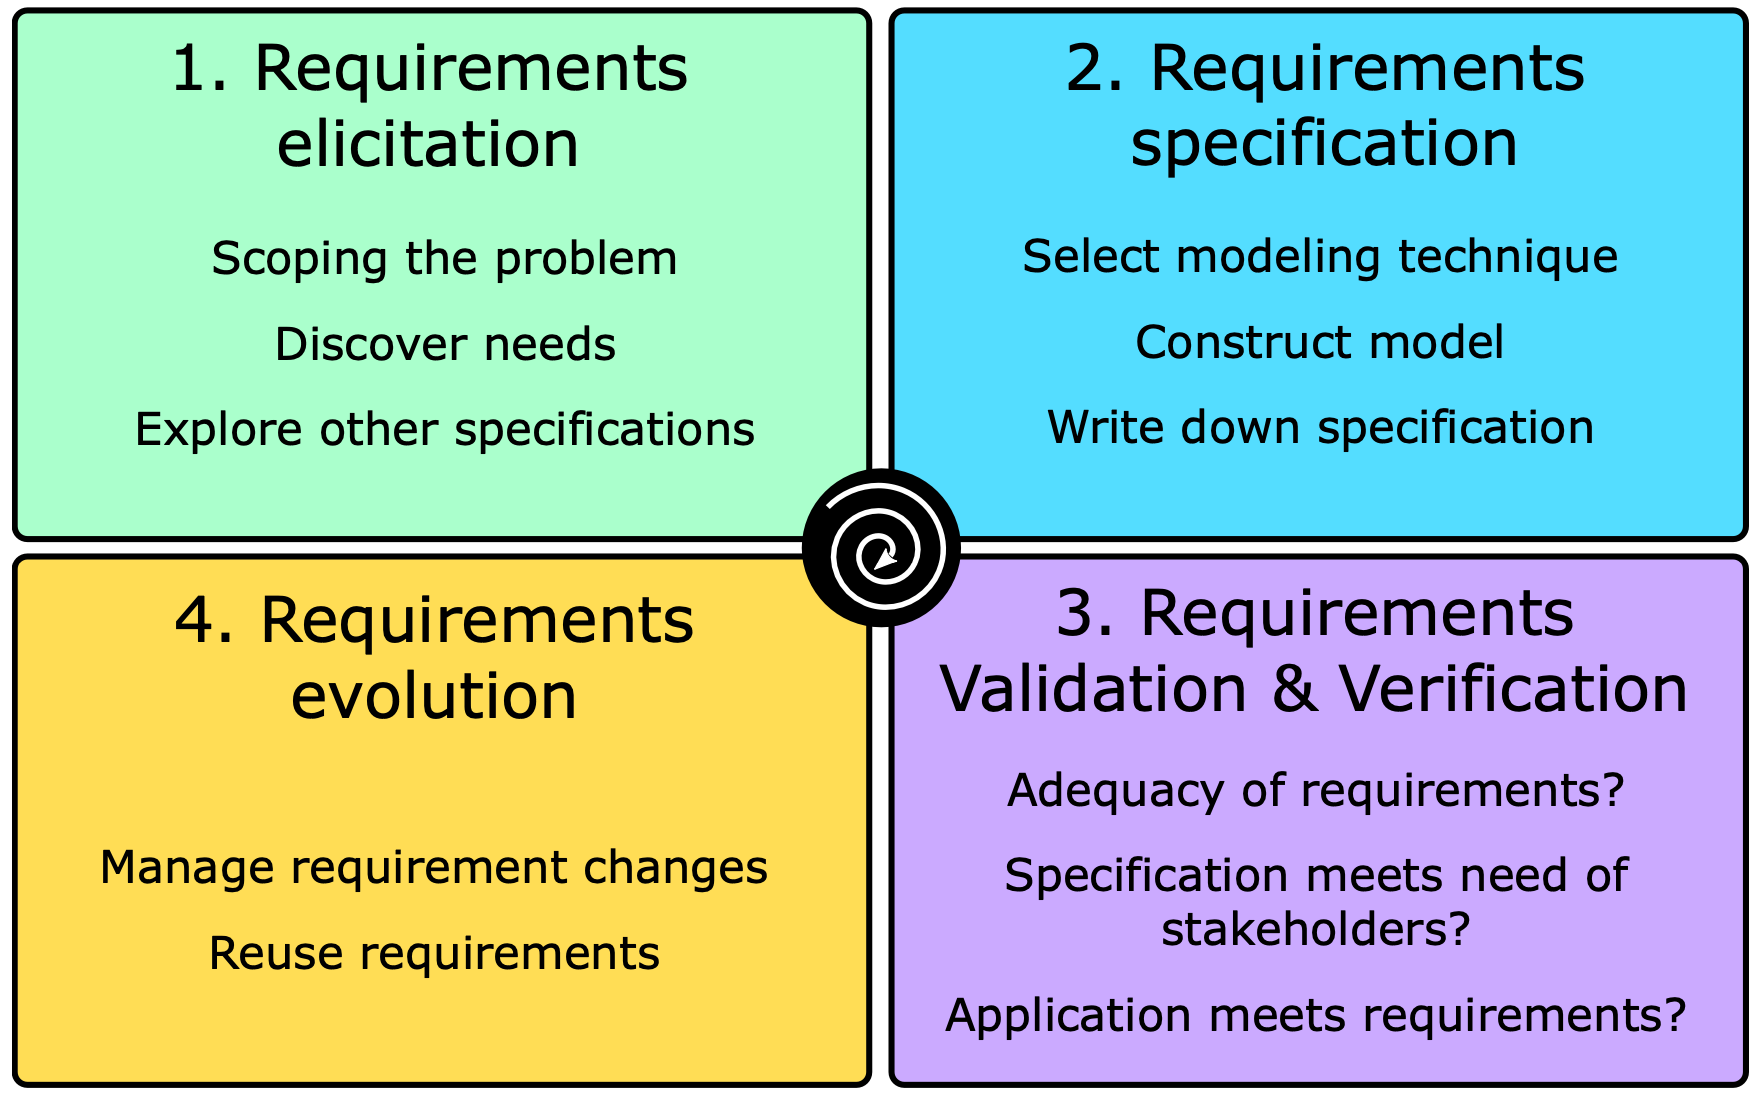
\includegraphics[scale=0.2]{requirements_main_activities.png}
\end{table}
\begin{table}[H]
\caption{Main Activities \& Documents}
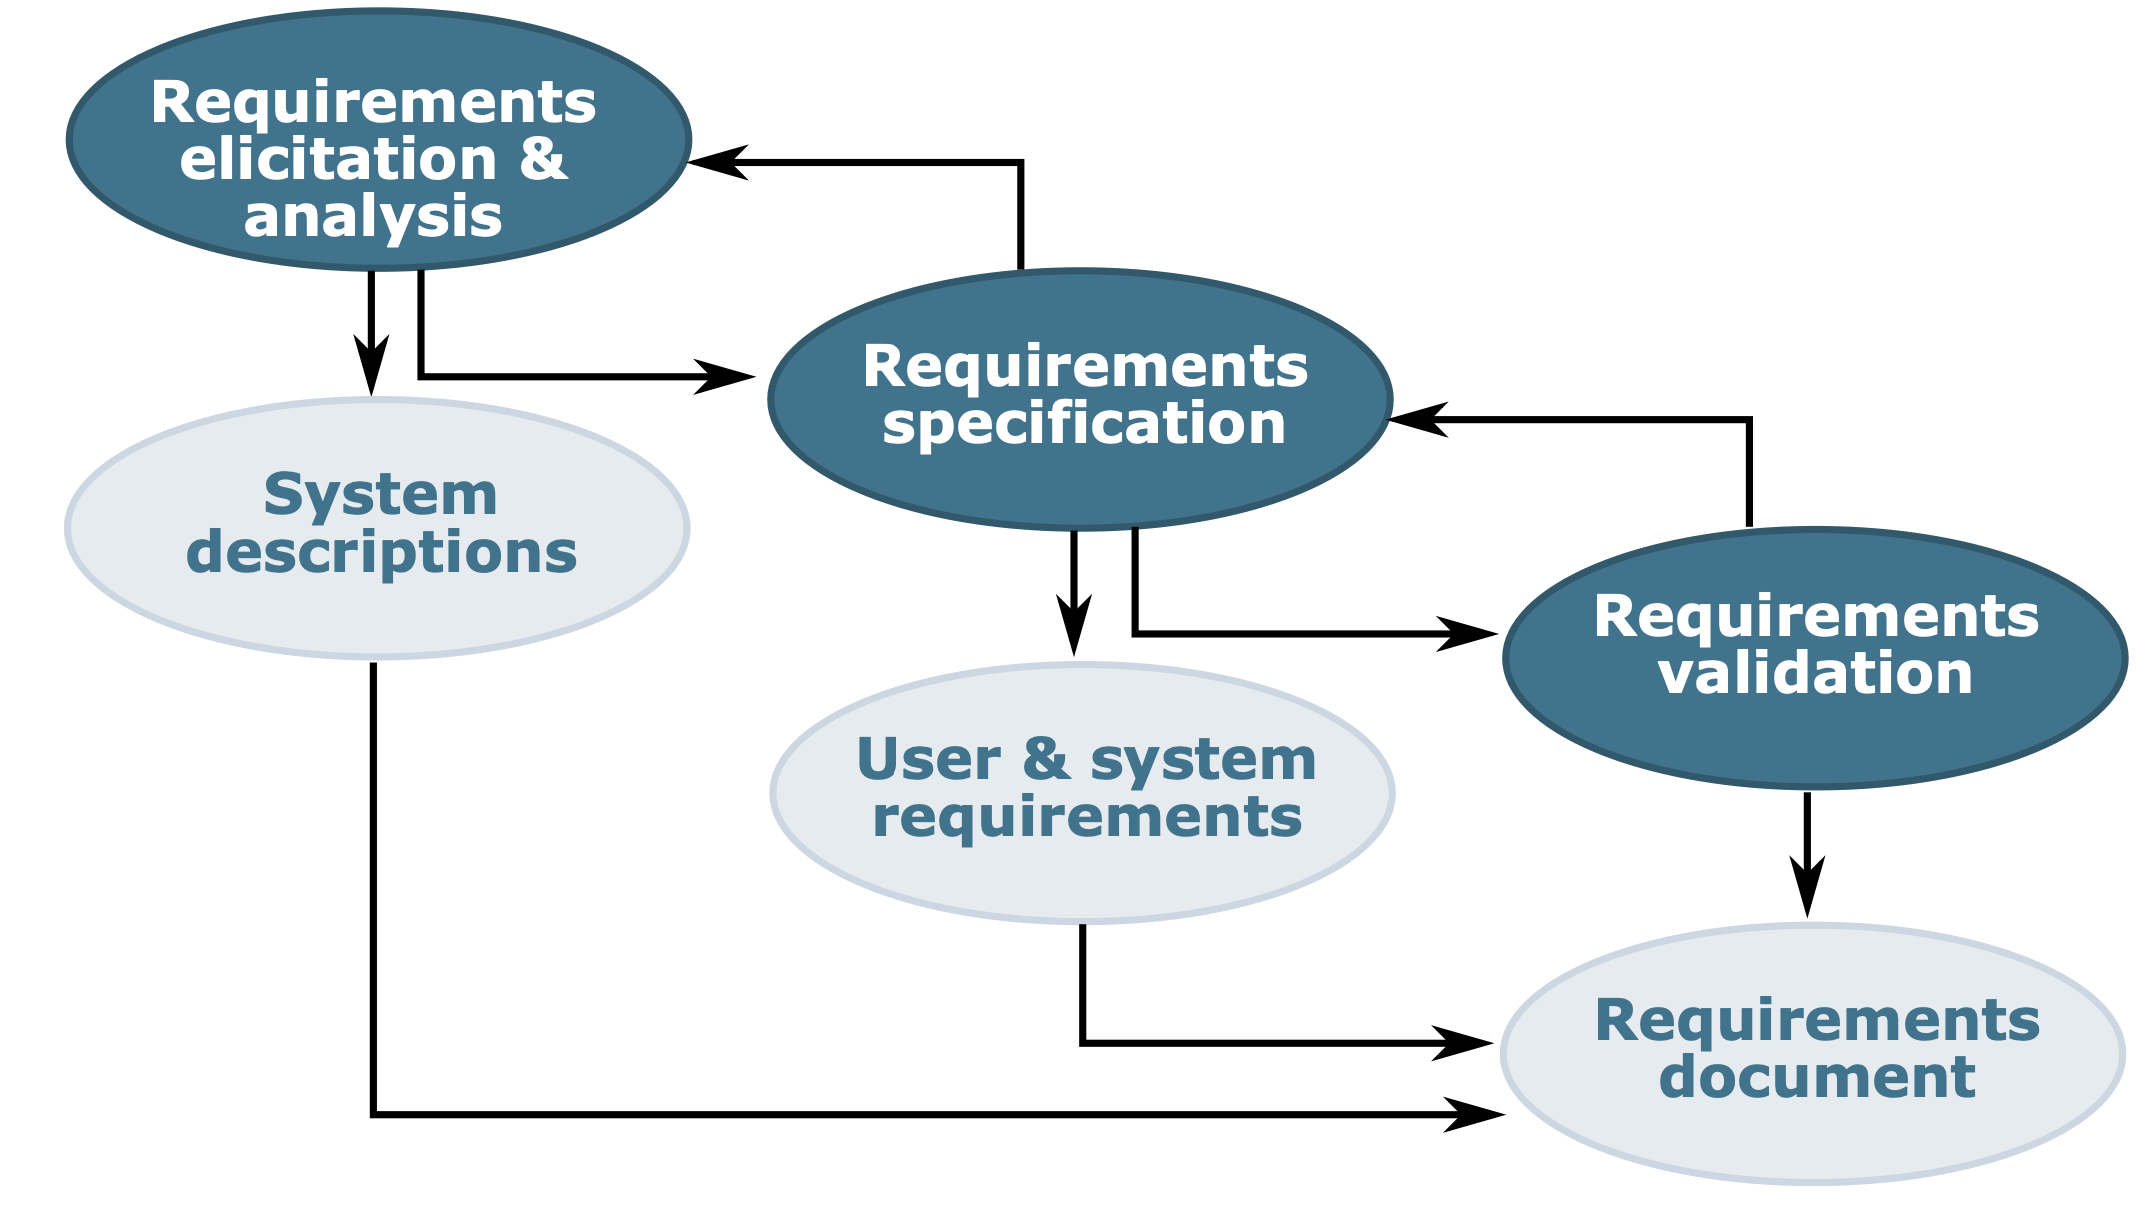
\includegraphics[scale=0.15]{requirements_documents.png}
\end{table}
\subsection{Requirements Elicitation}
$\bold{Problem}$: Kommunikation zwischen Kunden uns Entwicklern ist kompliziert, durch die nicht überschneidenden Expertisen
\subsubsection{Data gathering}
\begin{itemize}
	\item Background study
	\item Interviews
	\item Questionnaire
\end{itemize}
\subsubsection{Collaborative}
\begin{itemize}
	\item Brainstorming
	\item Joint application development (JAD) workshops
	\item Rapid application development (RAD) workshops
\end{itemize}
\subsubsection{Cognitive}
\begin{itemize}
	\item Repertory grids
	\item Card sorting
\end{itemize}
\subsubsection{Contextual}
\begin{itemize}
	\item Observation
	\item Protocol analysis
\end{itemize}
\subsubsection{Creativity}
\begin{itemize}
	\item Creativity workshops
	\item ContraVision
\end{itemize}
\subsection{Requirements Specification}
\subsubsection{Modeling techniques}
\begin{itemize}
	\item Natural language specification
		\begin{itemize}
			\item Easy Approach to Requirements Syntax (EARS) \newline
					(while, when, where, if then: shall)
			\item MoSCoW (Must, Should, Could \& Won't)
		\end{itemize}
	\item Structural modeling (what)
		\begin{itemize}
			\item Problem Frames
			\item Class diagrams
			\item Entity-Relationship (ER) diagrams 
		\end{itemize}
	\item Behavioural modeling (how)
		\begin{itemize}
			\item Use cases: semi-formal
			\item (Finite) state machines: formal
			\item Petri nets: formal
		\end{itemize}
	\item Goal modeling (why \& who)
		\begin{itemize}
			\item KOAS
			\item i*
		\end{itemize}
\end{itemize}
\begin{table}[H]
\caption{Problem diagram}
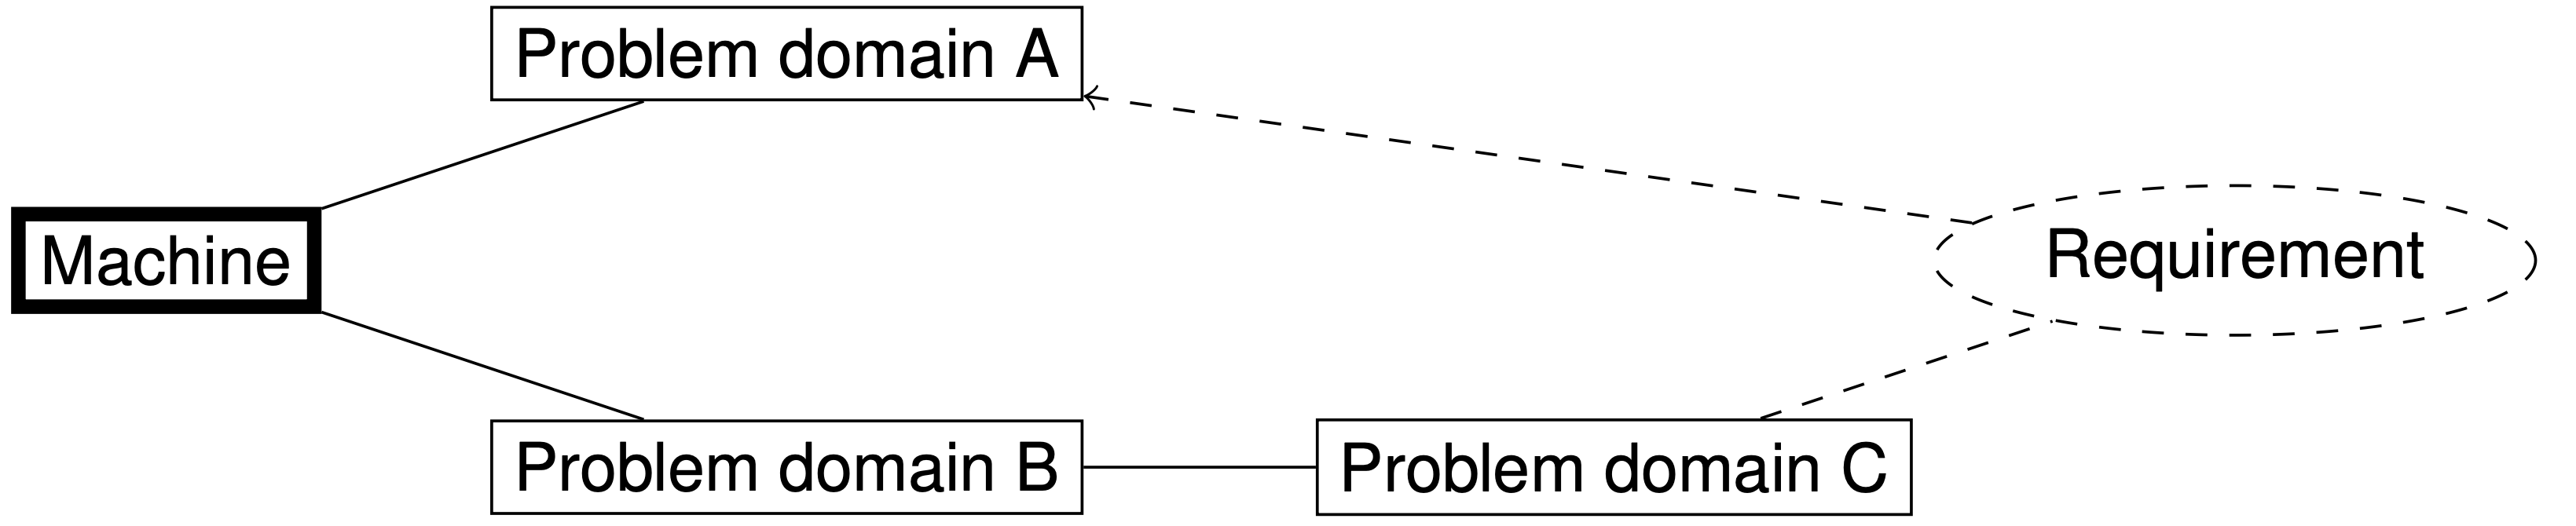
\includegraphics[scale=0.125]{Problem_diagram.png}
\end{table}
\begin{table}[H]
\caption{ER-diagram}
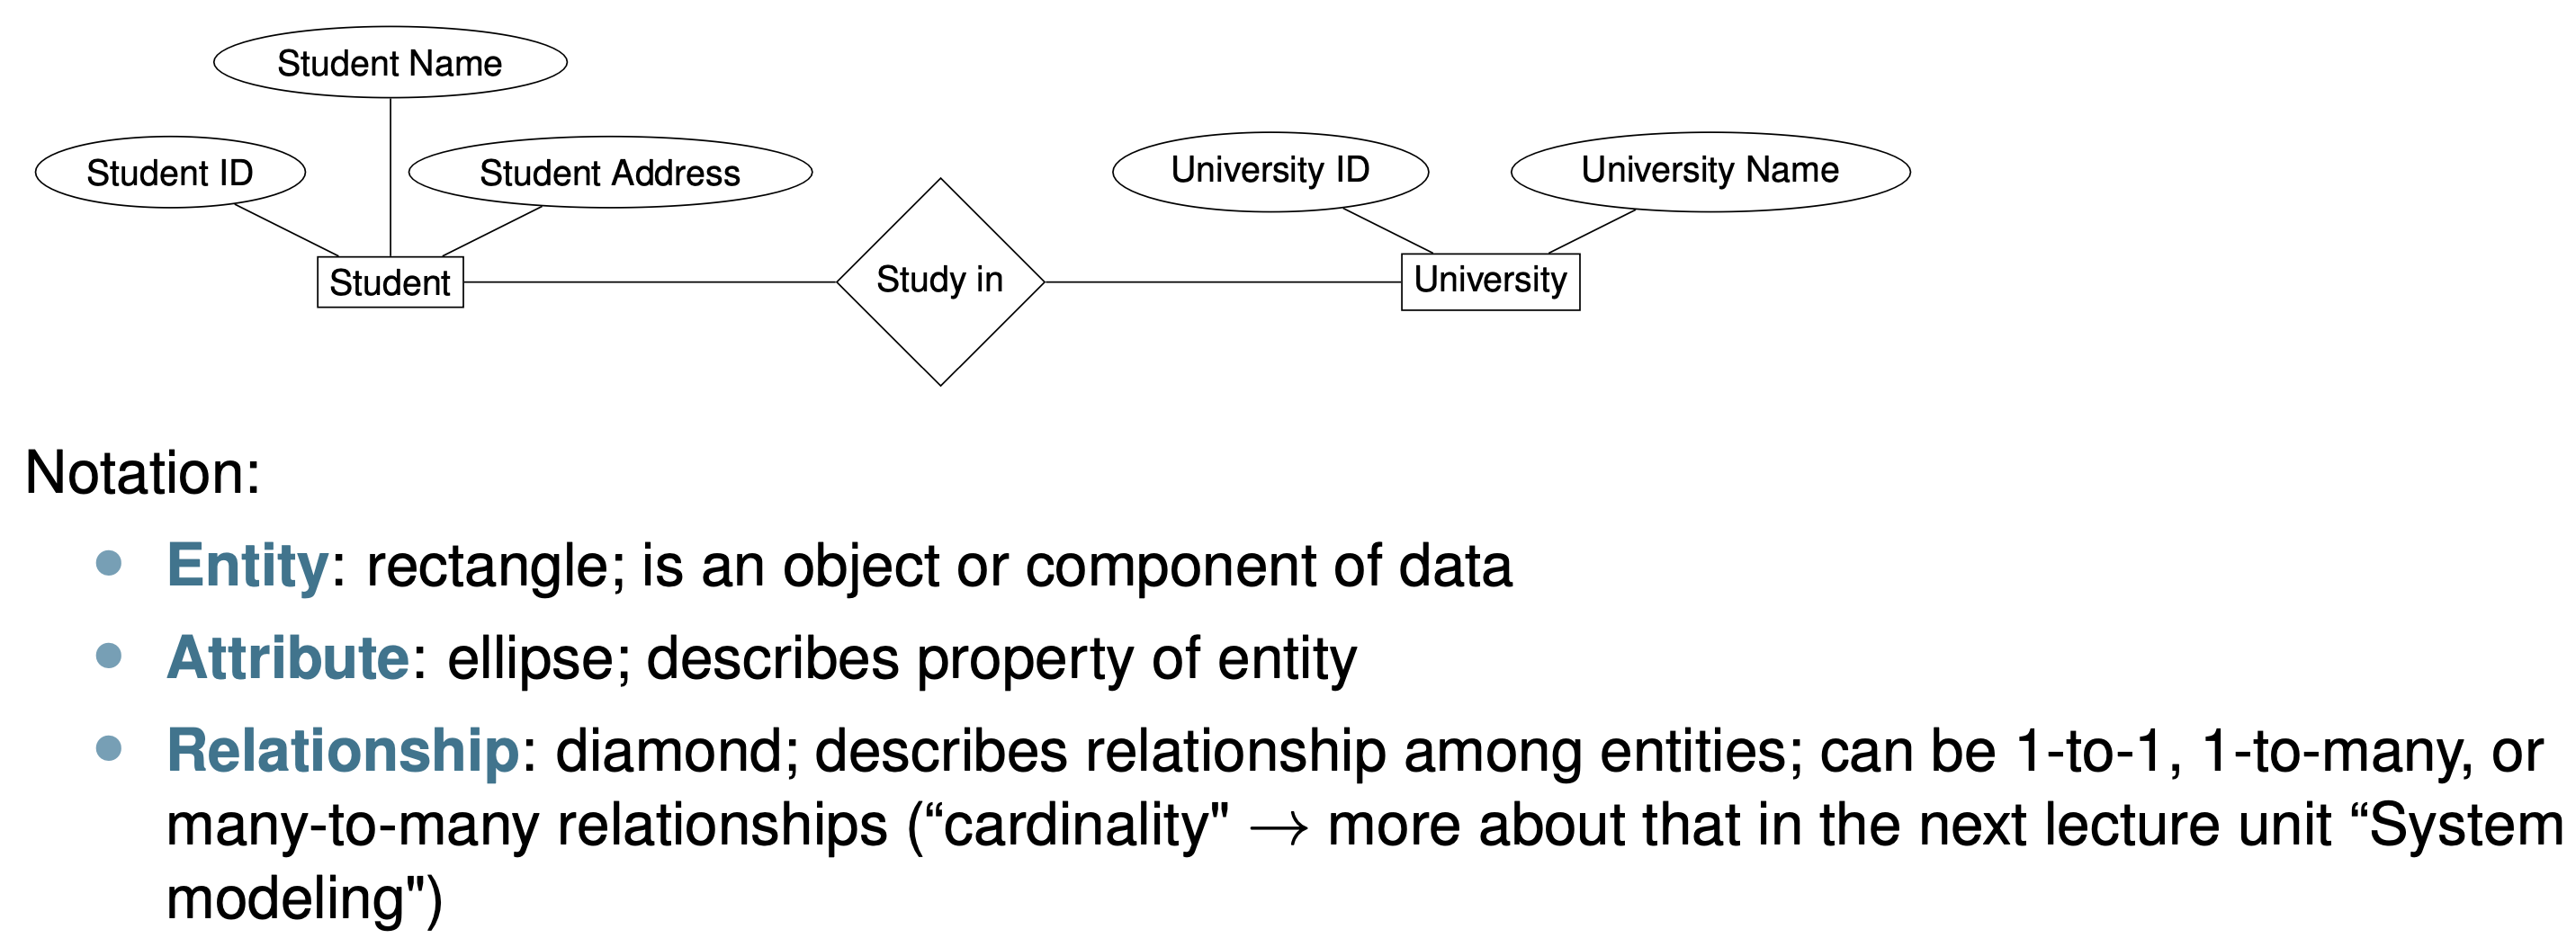
\includegraphics[scale=0.125]{ER_diagram_1.png}
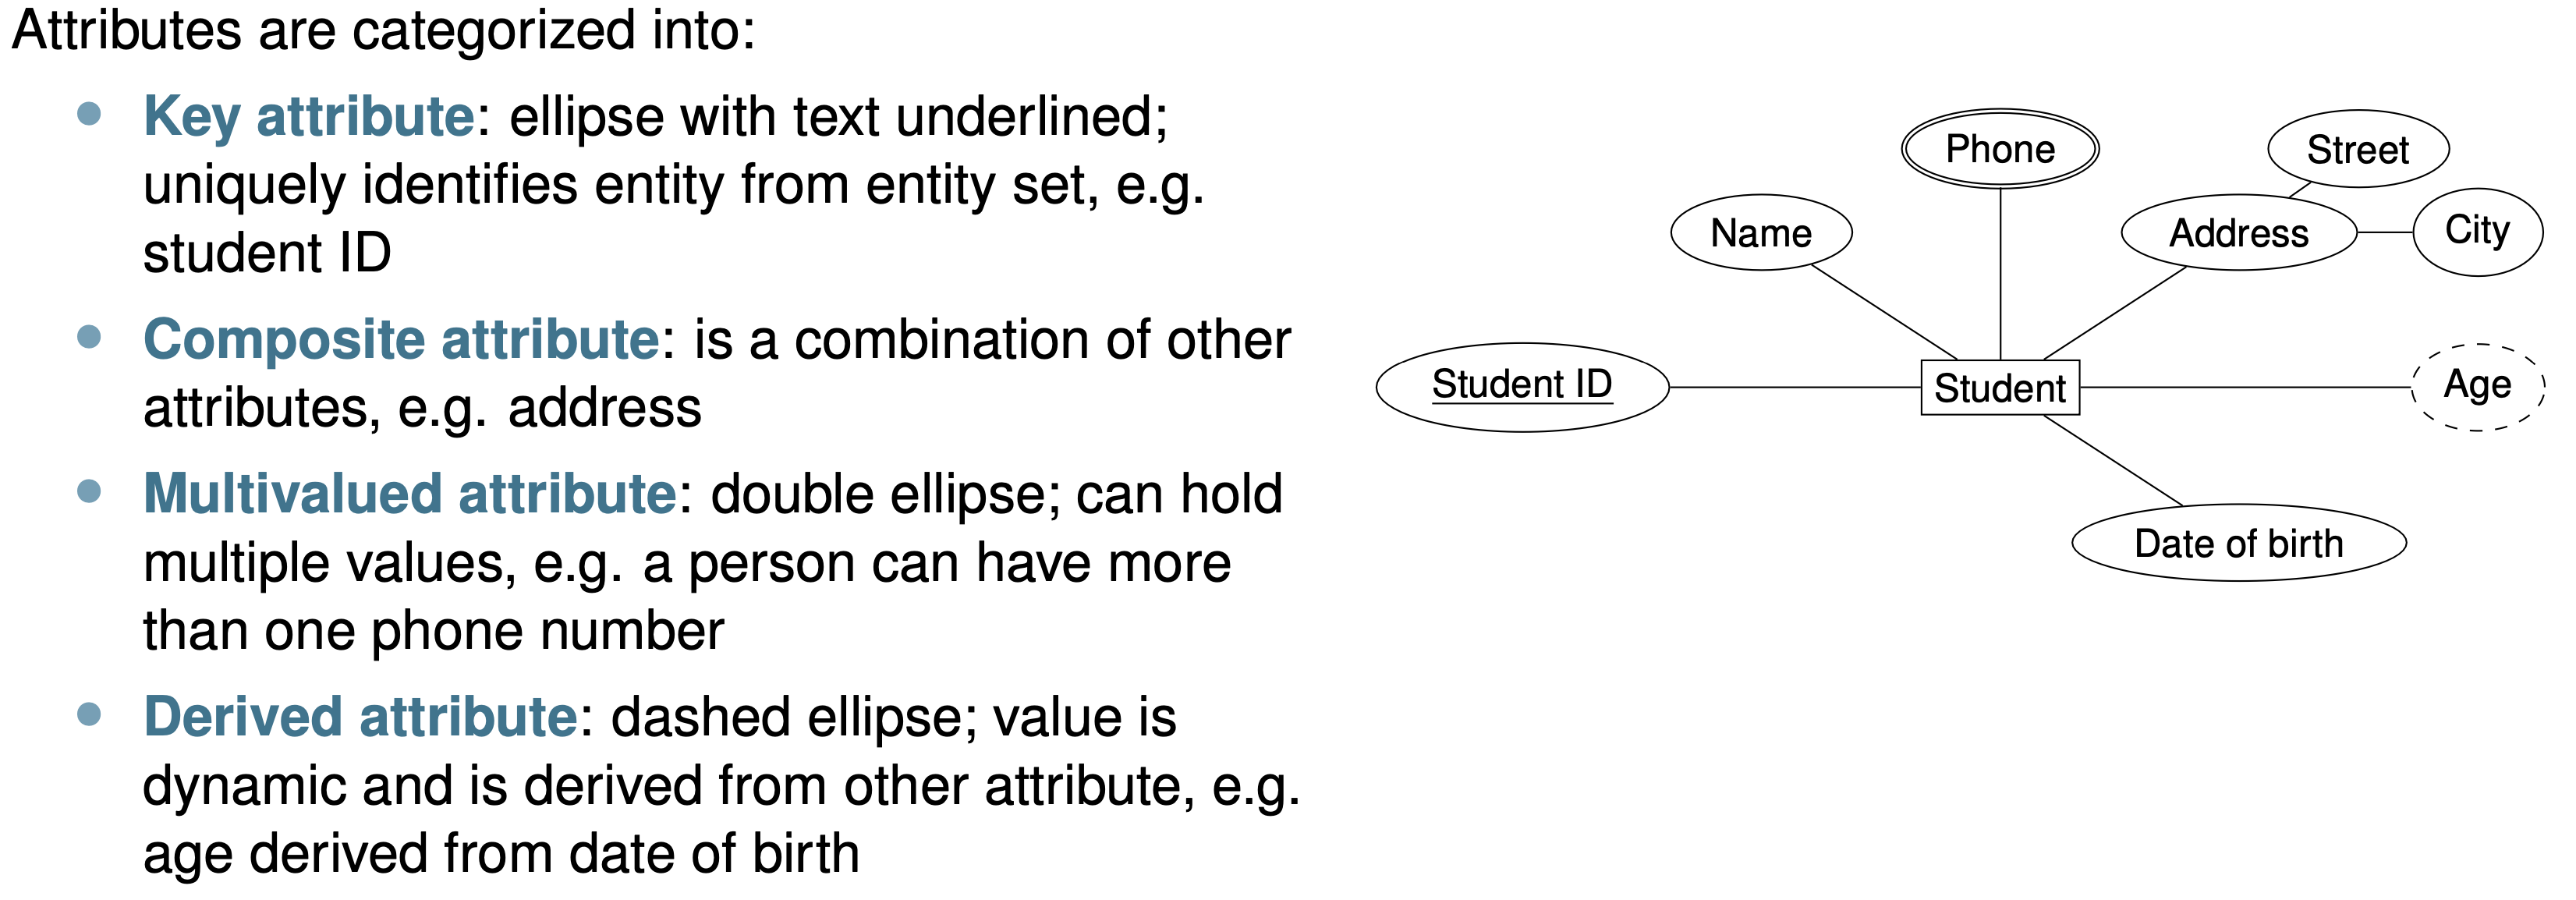
\includegraphics[scale=0.125]{ER_diagram_2.png}
\end{table}
\begin{table}[H]
\caption{Use case diagram}
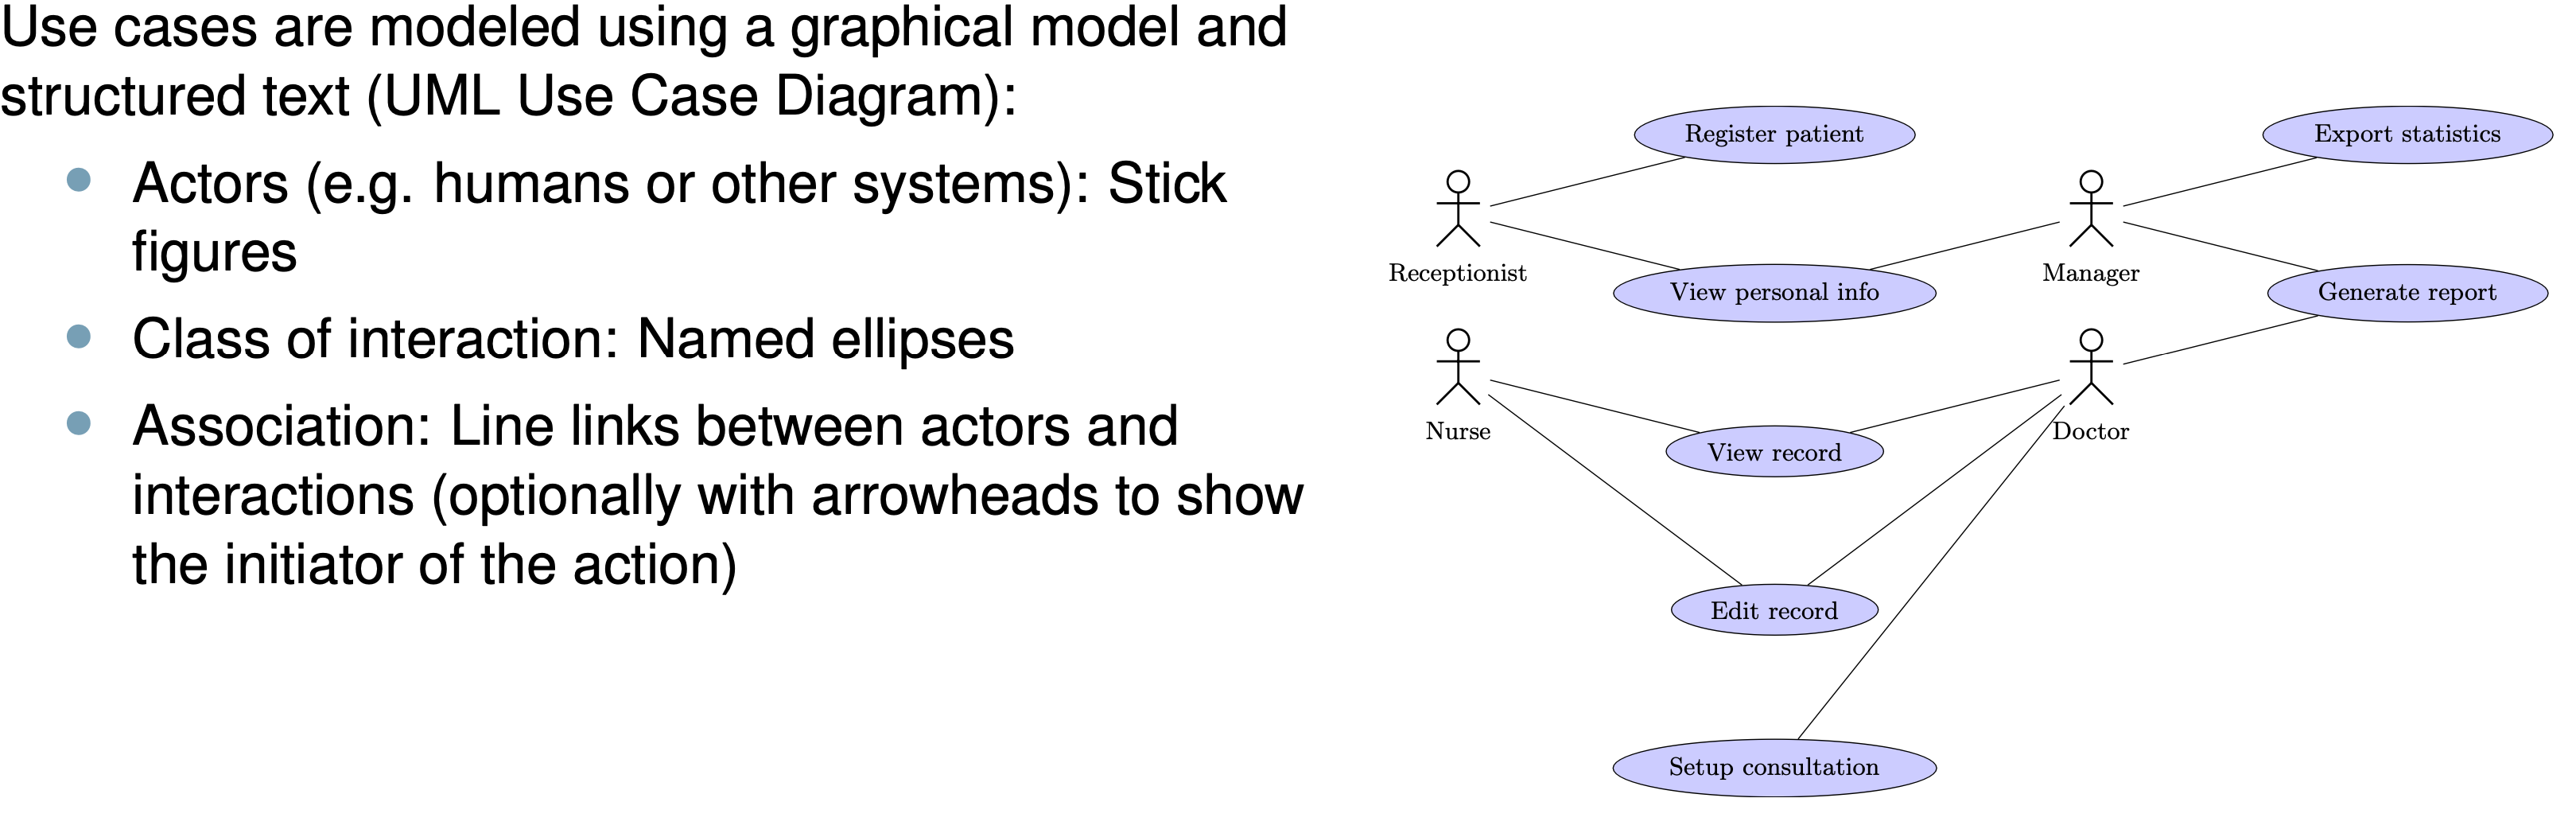
\includegraphics[scale=0.125]{Use_case_diagram.png}
\end{table}
\subsection{Agile Requirements Specification}

 
 
 
 
 